\documentclass{report}
% Maths Packages
\usepackage{mathtools, amsthm, amssymb, mathrsfs, interval, stmaryrd, centernot, esvect, cancel, commath, blkarray, empheq}
\usepackage{tabularx}
\usepackage{booktabs}
\usepackage{cellspace}
\setlength{\cellspacetoplimit}{5pt}
\setlength{\cellspacebottomlimit}{5pt}


% Sagemaths Formating Packages
\usepackage{listings}
\lstdefinelanguage{Sage}[]{Python}
{morekeywords={False,sage,True},sensitive=true}
\lstset{
  frame=none,
  showtabs=False,
  showspaces=False,
  showstringspaces=False,
  commentstyle={\ttfamily\color{dgreencolor}},
  keywordstyle={\ttfamily\color{dbluecolor}\bfseries},
  stringstyle={\ttfamily\color{dgraycolor}\bfseries},
  language=Sage,
  basicstyle={\fontsize{10pt}{10pt}\ttfamily},
  aboveskip=0.4em,
  belowskip=0.4em,
}

% TOC Packages
\usepackage{tocloft, titletoc, hyperref, bookmark}
% Formatting / Style Packages
\usepackage[T1]{fontenc}
\usepackage{geometry, subcaption, graphicx, fix-cm, accents, float, varwidth, soul, ulem, contour, multicol, enumitem}    
\usepackage[bottom]{footmisc}
\usepackage[x11names, table]{xcolor}
\usepackage[most, skins]{tcolorbox}
\usepackage{adjustbox}
\DeclareMathAlphabet{\mathmybb}{U}{bbold}{m}{n} % Indicatrices
\newcommand{\1}{\mathmybb{1}}

% Tikz
\usepackage{tikz, tkz-fct, tkz-euclide, tikz-cd, tkz-fct, pgfplots}
\pgfplotsset{compat=1.18}
\usetikzlibrary{
  angles, quotes, 3d, positioning,
  shapes,fit, arrows, arrows.meta, calc, 
  matrix, calligraphy, intersections, 
  quotes, patterns, patterns.meta, 
  decorations.pathreplacing, decorations.markings,decorations.pathmorphing,
}
\usepgfplotslibrary{fillbetween}
\tikzset{
  withparens/.style = {draw, outer sep=0pt,
    left delimiter= (, right delimiter=),
    above delimiter= (, below delimiter=),
    align=center},
  withbraces/.style = {draw, outer sep=0pt,
    left delimiter=\{, right delimiter=\},
    above delimiter=\{, below delimiter=\},
    align=center}
}
\tikzcdset{
  arrow style=tikz,
  diagrams={>={Straight Barb[scale=1]}},
}

% PAGE SETTINGS

\geometry{
  left=25mm, right=25mm, top= 15mm, bottom= 15mm,
  footskip=30pt
  }
\setlength{\parindent}{0cm}
\setlength{\parskip}{0cm}
\setlist[itemize]{itemsep=0pt, leftmargin=25pt}

\setlength{\cftbeforetoctitleskip}{0pt}
\setlength{\cftaftertoctitleskip}{0pt}

\setcounter{secnumdepth}{-1}

% STYLE
\definecolor{BrightBlue1}{RGB}{95, 150, 210}

\definecolor{BrightRed1}{RGB}{210, 95, 95}
\definecolor{BrightRed2}{RGB}{210, 115, 115}

\definecolor{DarkBlueX}{RGB}{43, 68, 92}
\definecolor{DarkBlue0}{RGB}{53, 78, 102}
\definecolor{DarkBlue1}{RGB}{83, 108, 132}
\definecolor{DarkBlue2}{RGB}{58, 94, 132}
\definecolor{DarkBlue3}{RGB}{90, 126, 162}

\definecolor{DarkGreen3}{RGB}{83, 132, 108}
\definecolor{DarkGreen2}{RGB}{58, 132, 94}
\definecolor{DarkGreen1}{RGB}{90, 162, 126}
\tcbset{shield externalize, enhanced, sharp corners, halign=center, center}

\definecolor{dblackcolor}{rgb}{0.0,0.0,0.0}
\definecolor{dbluecolor}{rgb}{0.01,0.02,0.7}
\definecolor{dgreencolor}{rgb}{0.2,0.4,0.0}
\definecolor{dgraycolor}{rgb}{0.30,0.3,0.30}
\newcommand{\dblue}{\color{dbluecolor}\bf}
\newcommand{\dred}{\color{dredcolor}\bf}
\newcommand{\dblack}{\color{dblackcolor}\bf}

%Underline settings
\setlength{\ULdepth}{2pt}
\contourlength{0.8pt}
\renewcommand{\underline}[1]{
  \uline{\phantom{#1}}%
  \llap{\contour{white}{#1}}%
}

%drop shadow southwest=black!100!black
\newcommand{\secstyle}[1]{\color{DarkBlue1}\fbox{#1}}
\newcommand{\subsecstyle}[1]{\color{DarkBlue2}\underline{#1}}
\newcommand{\subsubsecstyle}[2]{\color{DarkBlue3}\underline{#1}}

\newcommand{\chapterstyle}[1]{
    \setlength{\fboxsep}{0.3em}
    \setlength{\fboxrule}{3pt}
    \centering\vspace{-70pt}
    
    \color{DarkBlue1}\huge\fbox{\textbf{\textsc{#1}}}
}

\newcommand{\customBox}[2]{
    \tcbset{boxrule=1.5pt, boxsep=-0.2mm, colframe=DarkBlue1, colback=BrightBlue1!05}
    \begin{tcolorbox}[#1]
        \abovedisplayskip=0pt % remove vertical space above align
        #2
    \end{tcolorbox}
}

\makeatletter % Crée une trés grosse taille de police pour la page de garde
\newcommand\HUGE{\@setfontsize\Huge{40}{60}}
\makeatother   

\makeatletter
\newcommand\footnoteref[1]{\protected@xdef\@thefnmark{\ref{#1}}\@footnotemark}
\makeatother

% COMMANDS
% TOC
\renewcommand{\cftchapfont}{\large \bfseries \scshape}
\renewcommand{\cftsecfont}{}
\renewcommand{\contentsname}{\hfill
\setlength{\fboxsep}{0.3em}\setlength{\fboxrule}{3pt}\vspace{20pt}
   \color{DarkBlue1}\Huge
   \fbox{\textbf{\textsc{Table des matières}}}
   \hfill
}

% MATHS
\newcommand{\C}{\mathbb{C}}
\newcommand{\R}{\mathbb{R}}
\newcommand{\Q}{\mathbb{Q}}
\newcommand{\Z}{\mathbb{Z}}
\newcommand{\N}{\mathbb{N}}
\newcommand{\U}{\mathbb{U}}
\newcommand{\K}{\mathbb{K}}

\newcommand{\A}{\mathbf{\mathscr{A}}}
\newcommand{\B}{\mathbf{\mathscr{B}}}
\newcommand{\Fam}{\mathbf{\mathscr{F}}}
\renewcommand{\P}{\mathbf{\mathscr{P}}}

\renewcommand{\epsilon}{\varepsilon}
\renewcommand{\rho}{\varrho}

\newcommand{\E}{\mathbf{\mathcal{E}}}
\newcommand{\F}{\mathbf{\mathcal{F}}}
\newcommand{\Pow}{\mathbf{\mathcal{P}}}
\newcommand{\G}{\mathbf{\mathfrak{G}}}

\newcommand{\<}{\bigskip}
\newcommand{\+}{\par}

% Notation equality

\newcommand\notationEq{\stackrel{\mbox{
    \begin{tiny}  
        notation
    \end{tiny}    
}}{=}}

% INTERVALS

\intervalconfig{separator symbol =  \,; \,}

\newcommand{\ioo}[2]{\interval[open]{#1}{#2}}
\newcommand{\ioc}[2]{\interval[open left]{#1}{#2}}
\newcommand{\ico}[2]{\interval[open right]{#1}{#2}}
\newcommand{\icc}[2]{\interval{#1}{#2}}

\newcommand{\intioo}[2]{\left\rrbracket{#1}\;;\;{#2}\right\llbracket}
\newcommand{\intioc}[2]{\left\rrbracket{#1}\;;\;{#2}\right\rrbracket}
\newcommand{\intico}[2]{\left\llbracket{#1}\;;\;{#2}\right\llbracket}
\newcommand{\inticc}[2]{\left\llbracket{#1}\;;\;{#2}\right\rrbracket}

% EQUATIONS NOTES

\newcommand{\shorteqnote}[1]{ &  & \text{\small\llap{#1}}}
\newcommand{\longeqnote}[1]{& & \\ \notag&  &  &  &  & \text{\small\llap{#1}}}

% FUNCTIONS NOTATIONS

\newcommand{\inject}{\hookrightarrow} 
\newcommand{\surject}{\twoheadrightarrow}

% MOD NOTATION

\newcommand{\eqmod}[1]{\underset{#1}{\equiv}} 

% LINEAR ALGEBRA

\newcommand{\dotproduct}[2]{\left\langle\;\! #1 \;\! | \;\! #2 \;\! \right\rangle}
\newcommand{\vectNorm}[1]{\left\Vert#1 \right\Vert}

\newcommand{\Ker}[1]{\text{Ker}#1}
\newcommand{\Sp}[1]{\text{Sp}(#1)}
\renewcommand{\Im}[1]{\text{Im}#1}

\NewDocumentCommand{\opNorm}{sO{}m}{%
  \IfBooleanTF{#1}{% automatic scaling, use with care
    \left|\opnormkern\left|\opnormkern\left|
    #3
    \right|\opnormkern\right|\opnormkern\right|
  }{
    \mathopen{#2|\opnormkern #2|\opnormkern #2|}
    #3
    \mathclose{#2|\opnormkern #2|\opnormkern #2|}
  }%
}
\newcommand{\opnormkern}{\mkern-1.5mu\relax}% adjust for the font

% TOPOLOGY
\newcommand{\ball}{\mathscr{B}}

% CALCULUS
\newcommand{\partialD}[2]{\frac{\partial #1}{\partial #2}}

% GEOMETRY
\newcommand{\RightAgnle}[4][5pt]
{%
    \draw($#3!#1!#2$)-- ($#3!2! ($ ($#3!#1!#2$)!.5! ($#3!#1!#4$)$)$)-- ($#3!#1!#4$);
}

% PROBABILITIES
\newcommand{\probability}[1]{\mathbb{E} (#1)}
\newcommand{\expectancy}[1]{\mathbb{E} (#1)}
\newcommand{\variance}[1]{\mathbb{V} (#1)}
\newcommand{\covariance}[1]{\mathbb{C} (#1)}


\begin{document}
   \begin{titlepage}
   \begin{center}
       \vspace*{1cm}
       {
           \hfill
           \setlength{\fboxsep}{0.8em}\setlength{\fboxrule}{4pt}
           \color{DarkBlue1}\HUGE\fbox{\textbf{\textsc{Mathématiques}}}\hfill}

       \<
       {
       \color{DarkBlue1}\Large
       \textsc{Master}
       }
       \<

       \vspace{1.5cm}

       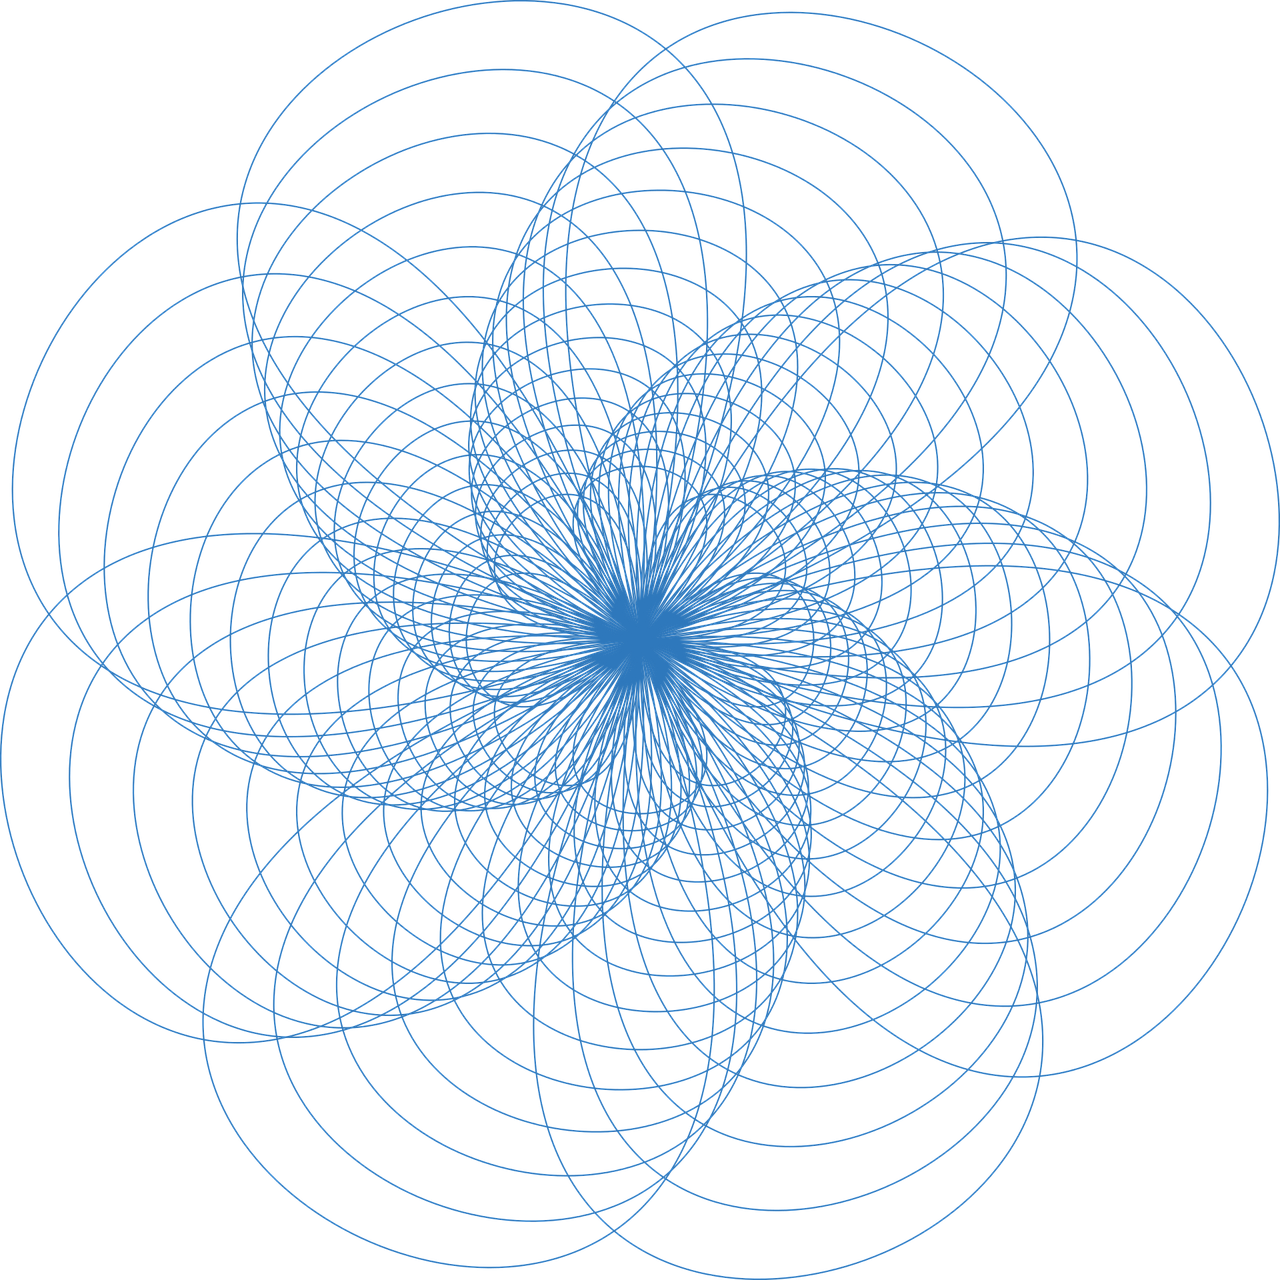
\includegraphics[width=0.9\textwidth]{Cover.png}

       \vfill

       \large
       \textsc{Université Paul Sabatier}\\
       \textsc{Année 2025-2027}
   \end{center}
\end{titlepage}

   \renewcommand{\cftchapfont}{\large \bfseries \scshape}
   \renewcommand{\cftsecfont}{}
   \renewcommand{\contentsname}{\hfill
   \setlength{\fboxsep}{0.3em}\setlength{\fboxrule}{3pt}\vspace{20pt}
   \color{DarkBlue1}\Huge
   \fbox{\textbf{\textsc{Table des matières}}}
   \hfill
   }
   
   \setcounter{tocdepth}{1}
   \tableofcontents

   \addcontentsline{toc}{chapter}{Analyse Fonctionnelle} % A FAIRE
   \chapter*{\chapterstyle{I --- Introduction}} % A REFAIRE
\addcontentsline{toc}{section}{Introduction} 

   \pagebreak    
   
   \addcontentsline{toc}{chapter}{Algèbre} % A FAIRE
   \chapter*{\chapterstyle{II --- Introduction}} % A REFAIRE
\addcontentsline{toc}{section}{Introduction} 

   \pagebreak    
   
   \addcontentsline{toc}{chapter}{Topologie Algébrique} % A FAIRE
   \chapter*{\chapterstyle{III --- Introduction}} % A REFAIRE
\addcontentsline{toc}{section}{Introduction} 

   \pagebreak     
   
   \addcontentsline{toc}{chapter}{Géométrie Différentielle} % A FAIRE
   \chapter*{\chapterstyle{IV --- Introduction}} % A REFAIRE
\addcontentsline{toc}{section}{Introduction} 

   \pagebreak  

   \addcontentsline{toc}{chapter}{Equations Différentielles Partielles} % A FAIRE
   \chapter*{\chapterstyle{V --- Introduction}} % A REFAIRE
\addcontentsline{toc}{section}{Introduction} 
Muni des corollaires du théorème des accroissements finis, on peut alors développer des méthodes pour résoudre des équations aux dérivées partielles simples, tout d'abord on appelle équations aux dérivées partielles une équation différentielle dont les solutions sont des fonctions inconnues dépendant de plusieurs variables vérifiant certaines conditions concernant leurs dérivées partielles. Par exemple l'équation suivante est une équation aux dérivées partielles:
\[
   \partialD{f}{x}(x, y) + \partialD{f}{y}(x, y) = 0   
\]
Ce chapitre à vocation à introduction et ne développera pas de théorie générale, simplement des méthodes élémentaires de resolution, souvent guidées. 
\subsection*{\subsecstyle{Cas simples à l'ordre 1{:}}}
On se donne \(f\) une fonction de classe \(\mathcal{C}^1(\R^2)\) et \(a \in \R\) et on considère tout d'abord les équations simples de la forme:
\[
   \partialD{}{x}(f) = a 
\]
Alors nécessairement, on a:
\[
   \partialD{}{x}(f - ax) = 0 
\]
Donc d'après le corollaire du théorème des accroissements finis, \(f - ax\) ne dépends pas de \(x\), pour une certaine fonction \(C \in \mathcal{C}^1(\R)\) on a donc:
\[
   f(x, y) = ax + C(y)
\]
On peut vérifier que réciproquement, cette fonction convient. Considérons un autre exemple moins trivial:
\[
   \partialD{}{x}(f) = h(x)   
\]
Alors on considère \(H\) une primitive de \(h\) et on peut alors écrire:
\[
   \partialD{}{x}(f - H(x)) = 0
\]
Et donc finalement d'aprés le corollaire du théorème:
\[
   f(x, y) = H(x) + C(y) 
\]
On vérifie à nouveau que réciproquement, cette fonction convient. On a ici illustré notre première méthode de résolution des cas simples d'équations aux dérivées partielles qui consiste à se ramener au corollaire du théorème
\subsection*{\subsecstyle{Cas simples à l'ordre 2{:}}}
On se donne \(f\) une fonction de classe \(\mathcal{C}^2(\R^2)\), on peut alors généraliser cette approche aux cas simples à l'ordre 2, par exemple:
\[
   \partialD{{}^2}{x^2}(f) = h(x)   
\]
Alors pour \(H\) une primitive de \(h\) on a nécessairement:
\[
   \partialD{}{x}(\partialD{}{x}(f) - H(x)) = 0 
\]
Donc d'aprés le corollaire du théorème:
\[
   \partialD{}{x}(f) = H(x) + C(y)
\]
Et on peut alors appliquer les méthodes de l'ordre 1 simplement pour conclure.

\subsection*{\subsecstyle{Changement de variable{:}}}
On considère \(f\) une fonction de classe \(\mathcal{C}^1(\R^2)\) qui vérifie une certaine équations aux dérivées partielles, ainsi qu'un \textbf{changement de variable} \(p : \R^2 \rightarrow \R^2\), ie un \(\mathcal{C}^1\)-difféomorphisme de \(\R^2\), alors on peut trovuer des solutions de l'équation sous l'une ou l'autre formes suivantes:
\[
   \begin{cases}
      f(x, y) = g(u, v) = (g \circ p)(x, y) \\
      f(u, v) = (f \circ p)(x, y) = g(x, y)\\
   \end{cases}
\]
On pourra alors facilement retrouver des solutions dans le systèmes de coordonées \((x, y)\) par composition.\<

\uline{Exemple 1:} On considère l'EDP:
\[
   \partialD{f}{x} - \partialD{f}{y} = 0   
\]
On pose alors \(p: (x, y) \mapsto (x + y, x - y)\) et on pose \(f(x, y) = (g \circ p)(x, y)\), alors d'aprés la règle de la chaîne, si \(f\) vérifie l'équation, on a nécessairement:
\[
   \partialD{g}{u} + \partialD{g}{v} - \partialD{g}{u} + \partialD{g}{v} = 2\partialD{g}{v} = 0
\]
On se ramène au corollaire du théorème, \(g\) ne dépend pas de sa variable \(v\) et donc:
\[
   g(u, v) = C(u)   
\]
Mais \(g(u, v) = f(x, y)\) et \(u = x + y\) donc finalement, on trouve:
\[
   f(x, y) = C(x + y)    
\]
Réciproquement, on montre facilement que cette fonction convient.

\chapter*{\chapterstyle{V --- Classification}} % A REFAIRE

   \pagebreak   

   \addcontentsline{toc}{chapter}{Probabilités} % A FAIRE
   \chapter*{\chapterstyle{VI --- Introduction}} % A REFAIRE
\addcontentsline{toc}{section}{Introduction} 

   \pagebreak   
\end{document}